\begin{figure*}[t]
\centering
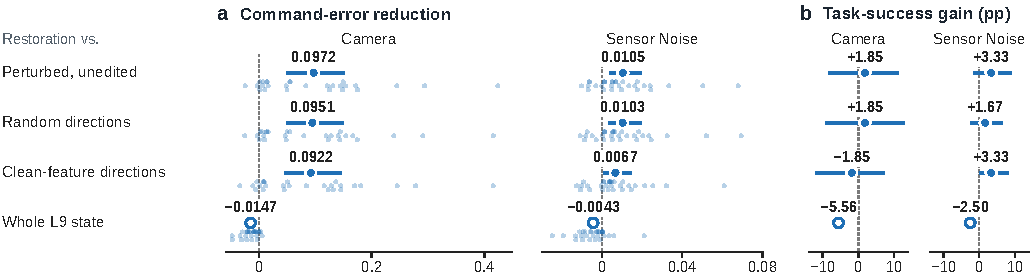
\includegraphics[width=\textwidth]{revised_figures/figure4_restoration_v3.pdf}
\caption{\textbf{Restoration against the unedited perturbed run, the two controls, and replacing the whole L9 state.}
Each row compares restoration with another run of the same cases (31 held-out tasks; Camera: 27 tasks, 96 cases; Sensor Noise: 30 tasks, 120 cases). Positive values favor restoration; negative values favor the other run, as for the whole L9 state on both measures. (a) Command error of the other run minus that of restoration: mean with simultaneous 95\% interval; small dots are tasks. Restoration lowers the command error of the unedited run in 25 of 27 and 24 of 30 tasks, and reduces it more than both controls, which also write less (edit size, Table~\ref{tab:restoration}). (b) Primary endpoint: success of restoration minus that of the other run, in percentage points, with intervals as in (a). The random-direction run under Camera and the clean-feature run under Sensor Noise succeed as often as the unedited run (Table~\ref{tab:restoration}), so their rows repeat its means. The whole-L9 run was not among the six prespecified comparisons, so it has no interval (open marks). Axes differ between families.}
\label{fig:native-restoration}
\end{figure*}
